\chapter{Preparing a high-quality PDF from LaTeX}\label{chap:PDFprep}
If the author chooses to complete the publications process using LaTeX\, the author must incorporate feedback and edits in to the LaTeX source files and prepare the final PDF, following these guidelines.

\section{PDF tagging}\label{sec:PDFtagging}
PDF tagging is a process whereby the components of the PDF document (headings, figures, tables, text) are marked so that a document reader can understand the document. This is useful when text to speech converters are being used. The process of tagging is also known as structuring, so that a tagged document might also be referred to as a structured document\footnote{This is a test}.

\LaTeX\ does not prepare a structured PDF document directly. Instead, we use the \texttt{accessibilityMeta} package to do this for us. This generates a tagged PDF that passes most automated document tests.

\section{Alternative text}\label{sec:Alttext}
Alternative text, or `Alt text', is a textual description of an equation, link or figure that can be used to replace the visual information in that element. This is often seen as a text `pop-up' in PDF readers. For example, passing the pointer over the following readers should reveal a pop-up:
\begin{equation}
\pdftooltip{a^2+b^2=c^2}{An equation}
\end{equation}

Alt text can be added after the PDF is compiled using a PDF editor such as Adobe's Acrobat Pro. Alternatively -- and probably best for ensuring that the final document is what the author intended -- it can be generated from within the source document using the \texttt{pdftooltip} environment from the \texttt{pdfcomment} package. The previous equation was generated using \verb?\pdftooltip{a^2+b^2=c^2}{An equation}?.

The same approach can be used to create alt text for images. For example, Figure \ref{fig:NRELimagesWithAltText} has been labeled with a tool tip. 

\begin{figure*}
          \begin{subfigure}[b]{.55\linewidth}
            \centering
		{\pdftooltip{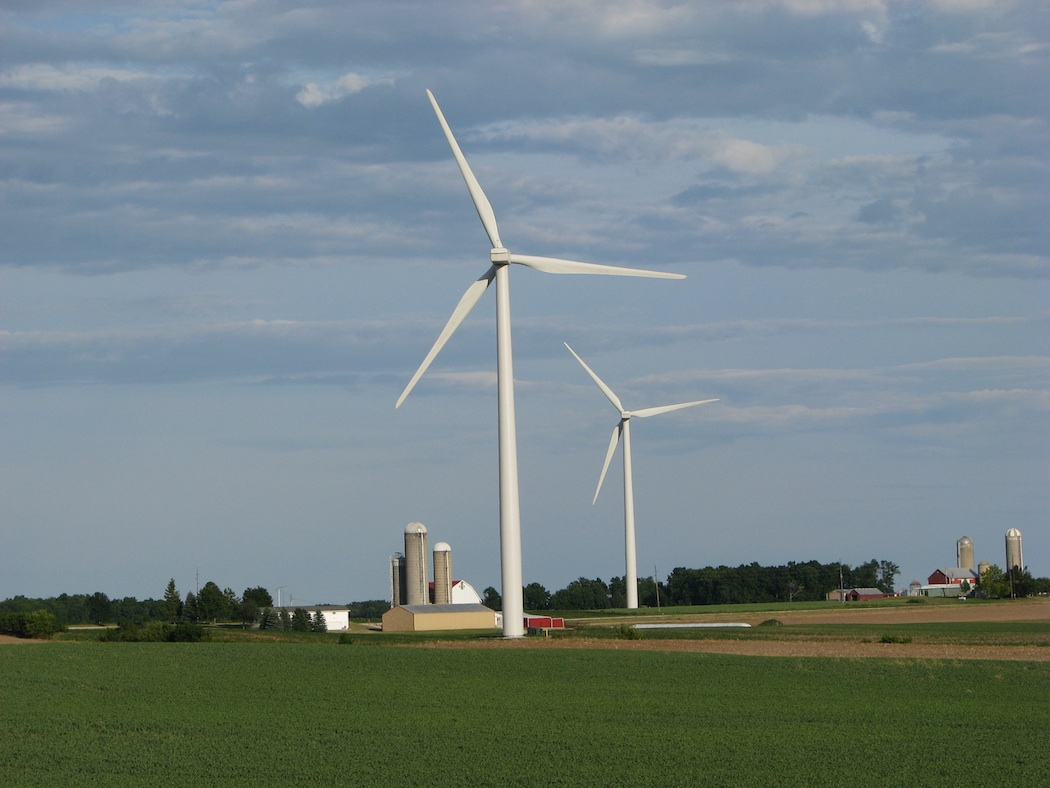
\includegraphics[height=2.5in]{files/21206}}{Wind turbines at the Forward Wind Energy Center in Fond du Lac and Dodge Counties, Wisconsin. (Photo by Ruth Baranowski / NREL)}}
            \caption{Wind turbines at the Forward Wind Energy Center in Fond du Lac and Dodge Counties, Wisconsin. (Photo by Ruth Baranowski / NREL).}\label{fig:21206WithAltText}
          \end{subfigure}%
          \begin{subfigure}[b]{.55\linewidth}
            \centering
		{\pdftooltip{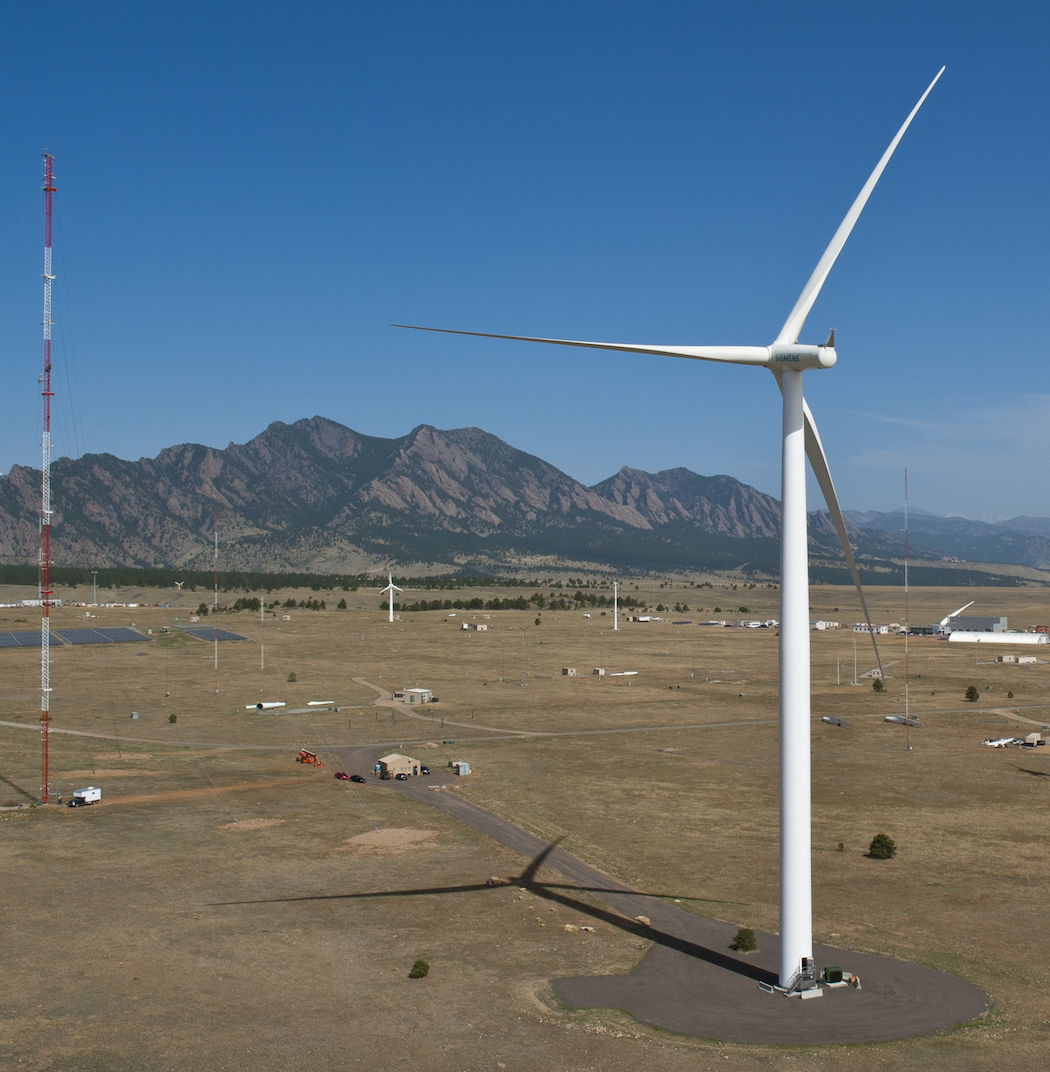
\includegraphics[height=2.5in]{files/20018}}{Aerial view of the National Wind Technology Center. (Photo by Dennis Schroeder / NREL)}}
            \caption{Aerial view of the National Wind Technology Center. (Photo by Dennis Schroeder / NREL)}\label{fig:20018WithAltText2}
          \end{subfigure}
          \caption{NREL images with Alt Text}\label{fig:NRELimagesWithAltText}
\end{figure*}

\section{Embedded fonts}
NREL requires that all fonts be embedded in the the final PDF. Check the PDF for embedded fonts using a PDF viewer. For example, in Adobe Acrobat Reader, look at the `fonts' tag of the document properties. If any fonts are not shown as being an \emph{embedded subset}, try the conversion again. 

Encapsulated postscript figures are particularly prone to having undefined fonts. Check by compiling the document in draft mode, and seeing if the fonts are still present in the output PDF. To fix this problem, change \emph{.eps} files to \emph{.png} files. To do this `on the fly', use this in the document's preamble:

\begin{lstlisting}
\usepackage{epstopdf}
\epstopdfDeclareGraphicsRule
 {.eps}{png}{.png}{convert eps:\SourceFile.\SourceExt png:\OutputFile}
\AppendGraphicsExtensions{.png}
\end{lstlisting}